
\documentclass{article}

\usepackage{graphicx}
\usepackage{subfig}
\usepackage{amsmath}
%\usepackage{amsmath,rotating}

\title{Laminar, Three-dimensional Pipe Flow}

\date{}

\begin{document}

\maketitle

\section{Introduction}
This case provides a description for three-dimensional laminar
pipe flow with constant properties, and a constant pressure gradient.

\section{Theory}
The three-dimensional geometry for this tutorial is captured in 
Figure~\ref{fig:geom}. Here, the cylindrical domain is defined by the 
length, $L$, and pipe diameter $d_o$, respectively. 

The left and right planes are open boundary conditions where a static pressure is specified. The configuration
can also be modeled with periodic planes with a specified body force. The outer pipe wall is a 
no-slip wall boundary condition.

\begin{figure}[!htbp]
  \centering
  {
   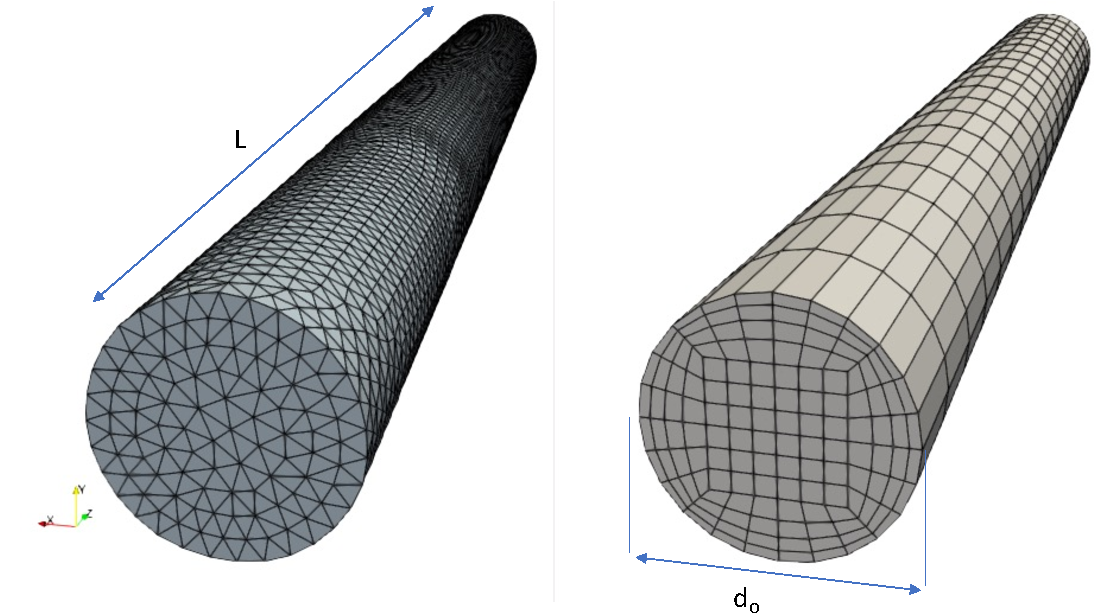
\includegraphics[height=2.0in]{images/3d_tet4_hex8_pipe_geom.pdf}
  }
  \caption{Three-dimensional pipe flow configuration of length $L$ and 
    diameter $d_o$ outlining the Tet4 (left) and Hex8 (right) topology.}
  \label{fig:geom}
\end{figure}

The variable-density low-Mach equation set is defined by the continuity and momentum equation.
Here, in cylindrical coordinates the axial coordinate
is $z$, the radial coordinate is $r$, and the azimuthal
coordinate is $\theta$.  The corresponding velocity definitions are as follows:
 $u_x$ is the axial velocity, $u_r$ is the radial velocity, and the azimuthal velocity is $u_\theta$. 
For an axisymmetric flow, derivatives in the $\theta-$direction are zero.

\noindent { Continuity Equation:}
\begin{equation}
     {{\partial \rho } \over {\partial t}}
   + \frac{1}{r}{{\partial r \rho u_r} \over {\partial r}} 
   + \frac{1}{r}{{\partial \rho u_\theta } \over {\partial \theta}} 
   + {{\partial \rho u_z } \over {\partial z}}
   = 0
\end{equation}

\noindent { Radial-Momentum Equation:}
\begin{eqnarray}
     \rho\left( {{\partial u_r} \over {\partial t}}
   + u_r {{\partial u_r} \over {\partial r}} 
   + \frac{u_\theta}{r} \frac{\partial u_r}{\partial \theta} -\frac{u_\theta^2}{r}
   + u_z\frac{\partial u_r}{\partial z} \right)
   + {{\partial P} \over {\partial r}} \\ \nonumber
   + \frac{1}{r}\frac{\partial r \tau_{rr}}{\partial r}
   + \frac{1}{r} \frac{\partial \tau_{r \theta}}{\partial \theta} - \frac{\tau_{\theta \theta}}{r}
   + \frac{\partial \tau_{rz}}{\partial z}
\end{eqnarray}

\noindent { Azimuthal-Momentum Equation:}
\begin{eqnarray}
     \rho\left( {{\partial u_\theta} \over {\partial t}}
   + u_r {{\partial u_\theta} \over {\partial r}} 
   + \frac{u_\theta}{r} \frac{\partial u_\theta}{\partial \theta} + \frac{u_r u_\theta}{r}
   + u_z\frac{\partial u_\theta}{\partial z}   \right)
   + \frac{1}{r}{{\partial P} \over {\partial \theta}} \\ \nonumber
   + \frac{1}{r^2}\frac{\partial r^2 \tau_{\theta r}}{\partial r}
   + \frac{1}{r} \frac{\partial \tau_{\theta \theta}}{\partial \theta} 
   + \frac{\partial \tau_{\theta z}}{\partial z}
\end{eqnarray}

\noindent { Axial-Momentum Equation:}
\begin{eqnarray}
     \rho\left( {{\partial u_z} \over {\partial t}}
   + u_r {{\partial u_z} \over {\partial r}} + \frac{u_\theta}{r} \frac{\partial u_z}{\partial \theta} 
   + u_z\frac{\partial u_z}{\partial z} \right)
   + {{\partial P} \over {\partial z}} \\ \nonumber
   + \frac{1}{r}\frac{\partial r \tau_{zr}}{\partial r}
   + \frac{1}{r} \frac{\partial \tau_{z \theta}}{\partial \theta}
   + \frac{\partial \tau_{zz}}{\partial z}
\end{eqnarray}

%
Above, the viscous stress terms are,
%
\begin{eqnarray}
  \tau_{rr} & = & \mu \left[ 2 {{\partial u_r} \over {\partial r}} 
              - {2 \over 3} \left( \frac{1}{r} \frac{\partial r u_r}{\partial r}
              + \frac{1}{r} \frac{\partial u_\theta}{\partial \theta}
              + \frac{\partial u_z}{\partial z} \right ) \right]  \\
  \tau_{\theta\theta} & = & \mu \left[ 2\frac{1}{r} \frac{\partial u_\theta}{\partial \theta} + 2 {u_r \over r} 
              - {2 \over 3} \left( \frac{1}{r} \frac{\partial r u_r}{\partial r}
              + \frac{1}{r} \frac{\partial u_\theta}{\partial \theta}
              + \frac{\partial u_z}{\partial z} \right ) \right]  \\
  \tau_{zz} & = & \mu \left[ 2 {{\partial u_z} \over {\partial z}} 
              - {2 \over 3} \left( \frac{1}{r} \frac{\partial r u_r}{\partial r}
              + \frac{1}{r} \frac{\partial u_\theta}{\partial \theta}
              + \frac{\partial u_z}{\partial z} \right ) \right]  \\
  \tau_{r\theta}  & = & \mu \left[ r \frac{\partial} {\partial r} \left( \frac{u_\theta}{r} \right) 
                             + \frac{1}{r} \frac{\partial u_r}{\partial u_\theta} \right] \\
  \tau_{rz} & = & \mu \left[ {{\partial u_r} \over {\partial z}} 
                         +   {{\partial u_z} \over {\partial r}} \right]  \\
  \tau_{z\theta} & = & \mu  \left[ {{\partial u_\theta} \over {\partial z}} + \frac{1}{r}\frac{\partial u_z}{\partial \theta} \right]
\end{eqnarray}
%
\subsection{Analytical Velocity Profile}
Given the assumptions provided in the introduction, the axial momentum equation reduces to,

\begin{align}
  \frac{d P}{dz} = \frac{1}{r}\frac{\partial r \tau_{\tau_{r z}}}{\partial r},
\label{eq:simpEq}
\end{align}
where $\tau_{r z} = \mu \frac{\partial u_z}{\partial r}$.
Integration once results in the following equation,
\begin{align}
  \frac{r^2}{2} \frac{d P}{dz} = r \mu \frac{\partial u_z}{\partial r} + k_1,
\label{eq:intOnce}
\end{align}
which, based on $\frac{\partial u_z}{\partial r} = 0$ at the centerline $r=0$, yields
$k_1$ = 0. A second integration results in,
\begin{align}
  u_z(r) = \frac{r^2}{4 \mu}\frac{d P}{dz} + k_2.
\label{eq:simpEqWithK}
\end{align}
Applying $u_z(r=R)$ = 0, yields the following expression for the axial velocity as a 
function of radial position,

\begin{align}
  u_z(r) = \frac{1}{4 \mu}\frac{d P}{dz}\left[ r^2 - R^2 \right].
\label{eq:simpleEqWithoutK}
\end{align}

The above equation can be used to determine the location at which 
the maximum velocity is found via solving $\frac{du_z}{dr} = 0$, or $u^{max}_z$ 
occurs at $r=0$. The functional form for the maximum velocity is,

\begin{align}
  u^{max}_x = -\frac{R^2}{4 \mu}\frac{d P}{d Z}.
\label{eq:uMax}
\end{align}

\section{Results}
Let us test a simulation in which the Reynolds number based on wall friction
velocity, $u^\tau$, and diameter of the pipe (0.02 $m$) is $Re^\tau = 20$. 
In this mesh configuration, the length $L$ is 0.2 m.
By constraining the Reynolds number, wall friction velocity, and density, 
the consistent viscosity is obtained via,

\begin{align}
  \mu = \frac{\rho u^\tau d_o}{Re^\tau}.
\label{eq:muForm}
\end{align}

To obtain the required pressure gradient, we exercise the relationship,

\begin{align}
  u^\tau = \sqrt{\frac{\tau_w}{\rho}},
\label{eq:tauWall}
\end{align}
along with global momentum balance,
%
\begin{align}
\int \frac{dP}{dz} dV = \int \tau_w dA,
\label{eq:balance}
\end{align}
with $dV = \pi r^2 L$ and $dA = 2\pi r L$, to obtain the relationship between
required pressure gradient and wall shear stress, $\frac{dP}{dz} = 2\frac{\tau_w}{r}$.

\subsection{Simulation Specification and Results}

Arbitrarily setting the density and wall friction velocity to unity, 
along with enforcing the diameter to be 2e-2 $m$, provides a required 
viscosity of $1e-3$ $Pa-s$ to obtain $Re^\tau$ = 20. Moreover, the required 
pressure gradient given our pipe length of 0.2 $m$ is 200. The mesh exercised 
activates a Tet4 topology, thereby exercising a linear underlying basis 
that yields a nominal second-order spatial accurate simulation.

In Figure~\ref{fig:results}, results are provided for the specifications
provided above. Note that although the analytical result was derived in 
cylindrical coordinates, the simulation is run in three-dimensional
Cartesian coordinates.

\begin{figure}[!htbp]
  \centering
  {
   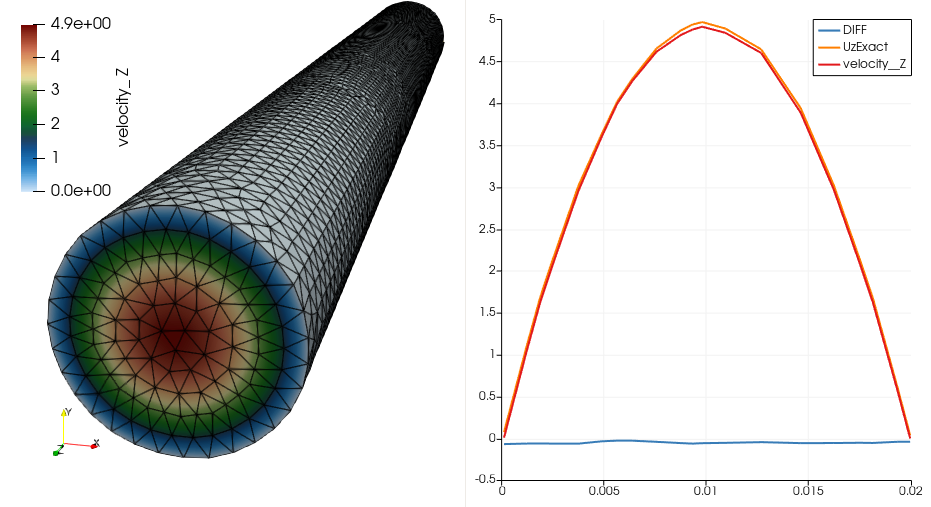
\includegraphics[height=2.0in]{images/3d_tet4_pipe_result.png}
  }
  \caption{Axial velocity shadings (left) and radial profile (roght) for 
    the $Re^\tau$ = 20 case.}
  \label{fig:results}
\end{figure}

\section{Discussion Points}

There are several interesting activities associated with this sample case 
including the following:

\begin{itemize}
	\item Ensure that derivation of Equation~\ref{eq:simpleEqWithoutK} is clear.
	\item Ensure that derivation of Equation~\ref{eq:uMax} is clear.
	\item Ensure that derivation of Equation~\ref{eq:balance} and the expression
           $\frac{dP}{dz} = 2\frac{\tau_w}{r}$ is clear.
	\item Explore the mesh and input file associated with this case.
	\item In Figure~\ref{fig:results}, it is noted that the difference between
          the analytical and simulation result is not zero. However, the underlying
          basis is a linear approach. Why are the results not exact as noted in the two-dimensional
          channel?
        \item Probe all degree-of-freedom results, i.e., velocity and pressure. What is of interest?
        \item When the simulation is run and wall shear stress is provided in the output file,
          what is the value? What are your findings?
        \item Are both provided meshes periodic in the axial direction?
        \item Comment on the role of nonlinear convergence on the overall accuracy of the result, i.e,
          axial velocity and pressure gradient?
          contrast the Hex8 and Tet4 simulation results.
        \item Run the Hex8 mesh simulation by modifying the input file to point to the Hex8 mesh. Compare and
          contrast the Hex8 and Tet4 simulation results. How is the mesh resolution for each near the wall?
\end{itemize}

\end{document}
